\chapter{Implementation}\label{ch:implementation}

This chapter details the implementation of our Retrieval-Augmented Generation system for validation rule discovery, examining the complete retrieval pipeline from data loading through hybrid scoring to user interface.

\section{System Architecture}

\subsection{Project Structure}

The implementation follows a modular architecture organized around the RAG pattern:

\begin{lstlisting}[
  language=bash, 
  caption={Project directory structure}, 
  label={lst:project-structure},
  basicstyle=\ttfamily\small,
  frame=single,
  backgroundcolor=\color{gray!5},
  xleftmargin=15pt,
  framexleftmargin=15pt,
  numbers=none
]
validation-rule-search/
├── app.py                         # Main Dash application
├── config.py                      # Configuration settings
├── rag/                           # RAG implementation
│   ├── embeddings/              # Embedding management
│   │   ├── manager.py         # Model operations
│   │   └── index.py           # Semantic search
│   └── search/                  # Search implementation
│       ├── retriever.py         # Hybrid retrieval
│       ├── config.py            # Search configuration
│       └── data.py              # Rule data loader
├── db/                            # Database layer
│   └── manager.py               # SQLite operations
└── data/
    └── validation_rules.csv       # Standardized corpus
\end{lstlisting}

\subsection{Architectural Overview}

The system implements a monolithic architecture where all components operate within a single Python process. This design eliminates network overhead between components and ensures deterministic behavior required for banking compliance. The retrieval pipeline processes queries through three parallel signals—semantic, BM25, and fuzzy—combining their normalized scores for final ranking.

\section{Core RAG Components}

\subsection{Embedding Manager}

The \texttt{EmbeddingManager} handles transformer-based embedding generation with attention-aware pooling, critical for accurate semantic representations:

\begin{lstlisting}[
  language=Python, 
  caption={Attention-aware mean pooling for embeddings}, 
  label={lst:mean-pooling},
  basicstyle=\ttfamily\footnotesize,
  keywordstyle=\color{blue}\bfseries,
  commentstyle=\color{green!50!black},
  stringstyle=\color{red!60!black},
  frame=lines,
  backgroundcolor=\color{gray!5},
  xleftmargin=15pt,
  framexleftmargin=15pt,
  numbers=left,
  numberstyle=\tiny\color{gray},
  numbersep=5pt
]
def _mean_pooling(self, model_output, attention_mask):
    """Apply attention-mask-aware mean pooling."""
    token_embeddings = model_output.last_hidden_state
    mask = attention_mask.unsqueeze(-1).to(
        dtype=token_embeddings.dtype
    )
    # Sum only non-padding tokens
    sum_embeddings = (token_embeddings * mask).sum(dim=1)
    token_counts = mask.sum(dim=1).clamp(min=1e-9)
    return sum_embeddings / token_counts

def generate_embeddings(self, texts, batch_size=32, 
                       use_cache=True):
    """Generate L2-normalized embeddings for texts."""
    if isinstance(texts, str):
        texts = [texts]
    
    embeddings = []
    for i in range(0, len(texts), batch_size):
        batch = texts[i:i + batch_size]
        
        # Check cache first
        uncached = []
        for t in batch:
            if use_cache and t in self._embedding_cache:
                embeddings.append(self._embedding_cache[t])
            else:
                uncached.append(t)
        
        if uncached:
            # Encode batch
            encoded = self.tokenizer(
                uncached, padding=True, truncation=True,
                return_tensors='pt', max_length=512
            ).to(self.device)
            
            with torch.no_grad():
                model_output = self.model(**encoded)
                pooled = self._mean_pooling(
                    model_output, 
                    encoded["attention_mask"]
                )
                # L2 normalize for cosine similarity
                normalized = F.normalize(pooled, p=2, dim=1)
            
            for j, t in enumerate(uncached):
                vec = normalized[j].cpu()
                if use_cache:
                    self._embedding_cache[t] = vec
                embeddings.append(vec)
    
    return torch.stack(embeddings).numpy()
\end{lstlisting}

\subsection{Embedding Index}

The \texttt{EmbeddingIndex} maintains pre-computed embeddings and performs efficient semantic search:

\begin{lstlisting}[
  language=Python, 
  caption={Semantic search via cosine similarity}, 
  label={lst:semantic-search},
  basicstyle=\ttfamily\footnotesize,
  keywordstyle=\color{blue}\bfseries,
  commentstyle=\color{green!50!black},
  stringstyle=\color{red!60!black},
  frame=lines,
  backgroundcolor=\color{gray!5},
  xleftmargin=15pt,
  framexleftmargin=15pt,
  numbers=left,
  numberstyle=\tiny\color{gray}
]
def search(self, query: str, top_k: int = 5):
    """Retrieve most similar rules to query."""
    # Encode query (manager ensures L2 normalization)
    query_emb = self.embedding_manager\
                    .generate_embeddings(query)[0]
    
    # Cosine similarity via dot product 
    # (vectors are normalized)
    sims = self.embeddings @ query_emb
    
    # Efficient partial sort for top-k
    k = min(top_k, len(self.metadata))
    top_idx = np.argpartition(-sims, k - 1)[:k]
    top_idx = top_idx[np.argsort(-sims[top_idx])]
    
    results = [(self.metadata[i], float(sims[i])) 
               for i in top_idx]
    return results
\end{lstlisting}

\subsection{Index Construction}

The system builds two indices at startup in parallel—semantic and BM25. Fuzzy matching requires no index as it operates directly on rule names at query time:

\begin{lstlisting}[
  language=Python, 
  caption={Parallel index construction at startup}, 
  label={lst:parallel-indices},
  basicstyle=\ttfamily\footnotesize,
  keywordstyle=\color{blue}\bfseries,
  commentstyle=\color{green!50!black},
  stringstyle=\color{red!60!black},
  frame=lines,
  backgroundcolor=\color{gray!5},
  xleftmargin=15pt,
  framexleftmargin=15pt,
  numbers=left,
  numberstyle=\tiny\color{gray}
]
def _build_indices(self):
    """Build semantic and BM25 indices in parallel.
    Note: Fuzzy matching needs no index 
          (computed at query time)."""
    
    def build_embedding_index():
        self.embedding_index = EmbeddingIndex(
            self.embedding_manager
        )
        self.embedding_index.add_rules(self.rules)
        logger.info(f"Embedding index built with "
                   f"{len(self.rules)} rules")
    
    def build_bm25_index():
        # Extract and tokenize keywords
        corpus = [r.get("keywords", "") 
                 for r in self.rules]
        tokenized = [kw.replace(",", " ").split() 
                    if kw else [] 
                    for kw in corpus]
        
        if tokenized and any(len(toks) > 0 
                           for toks in tokenized):
            self.bm25_index = BM25Okapi(tokenized)
            self._bm25_keywords_len = len(tokenized)
            logger.info(f"BM25 index built with "
                       f"{len(tokenized)} docs")
    
    # Execute in parallel for faster startup
    with ThreadPoolExecutor() as executor:
        futures = [
            executor.submit(build_embedding_index),
            executor.submit(build_bm25_index)
        ]
        for f in futures:
            f.result()
\end{lstlisting}

\subsection{Three Retrieval Signals}

The retriever implements three complementary scoring mechanisms:

\begin{lstlisting}[
  language=Python, 
  caption={Three retrieval signals implementation}, 
  label={lst:three-signals},
  basicstyle=\ttfamily\footnotesize,
  keywordstyle=\color{blue}\bfseries,
  commentstyle=\color{green!50!black},
  stringstyle=\color{red!60!black},
  frame=lines,
  backgroundcolor=\color{gray!5},
  xleftmargin=15pt,
  framexleftmargin=15pt,
  numbers=left,
  numberstyle=\tiny\color{gray}
]
def _semantic_scores(self, query: str, rules: List[dict]):
    """Compute semantic similarity scores 
       using embeddings."""
    if self.embedding_index is None:
        return {r["rule_id"]: 0.0 for r in rules}
    
    # Get all similarities from embedding index
    results = self.embedding_index.search(
        query, top_k=len(rules)
    )
    by_id = {r["rule_id"]: float(score) 
            for r, score in results}
    return {r["rule_id"]: by_id.get(r["rule_id"], 0.0) 
            for r in rules}

def _bm25_scores(self, query: str, rules: List[dict]):
    """Compute BM25 keyword matching scores."""
    if self.bm25_index is None:
        return {r["rule_id"]: 0.0 for r in rules}
    
    # Tokenize query same as corpus
    q_tokens = query.replace(",", " ").split()
    scores = self.bm25_index.get_scores(q_tokens)
    
    # Map scores to rule IDs
    id_to_pos = {r["rule_id"]: i 
                for i, r in enumerate(self.rules)}
    out = {}
    for r in rules:
        pos = id_to_pos.get(r["rule_id"])
        out[r["rule_id"]] = float(scores[pos]) \
                           if pos else 0.0
    return out

def _fuzzy_scores(self, query: str, rules: List[dict]):
    """Compute fuzzy string matching on rule names 
       (no index required)."""
    out = {}
    for r in rules:
        name = r.get("rule_name", "") or ""
        # Partial ratio finds best substring match
        score = fuzz.partial_ratio(
            query.lower(), name.lower()
        )
        out[r["rule_id"]] = float(score) / 100.0
    return out
\end{lstlisting}

\subsection{Hybrid Score Fusion}

The system combines three signals with max normalization and convex weights:

\begin{lstlisting}[
  language=Python, 
  caption={Hybrid score computation with normalization}, 
  label={lst:hybrid-scoring},
  basicstyle=\ttfamily\footnotesize,
  keywordstyle=\color{blue}\bfseries,
  commentstyle=\color{green!50!black},
  stringstyle=\color{red!60!black},
  frame=lines,
  backgroundcolor=\color{gray!5},
  xleftmargin=15pt,
  framexleftmargin=15pt,
  numbers=left,
  numberstyle=\tiny\color{gray}
]
def _normalize_per_prompt(self, scores: Dict[str, float]):
    """Normalize scores to [0, 1] relative to max."""
    if not scores:
        return scores
    mx = max(scores.values())
    if mx <= 0:
        return {k: 0.0 for k in scores}
    return {k: v / mx for k, v in scores.items()}

def _hybrid_scores(self, query: str, rules: List[dict]):
    """Weighted combination of three normalized signals."""
    # Get normalized scores from each signal
    sem = self._normalize_per_prompt(
        self._semantic_scores(query, rules)
    )
    bm25 = self._normalize_per_prompt(
        self._bm25_scores(query, rules)
    )
    fz = self._normalize_per_prompt(
        self._fuzzy_scores(query, rules)
    )
    
    # Ensure weights sum to 1.0 (convex combination)
    w_sem = max(self.config.semantic_weight, 0.0)  # 0.80
    w_kw = max(self.config.bm25_weight, 0.0)       # 0.10
    w_fz = max(self.config.fuzzy_weight, 0.0)      # 0.10
    sw = w_sem + w_kw + w_fz
    if sw == 0:
        w_sem = w_kw = w_fz = 1.0 / 3.0
    else:
        w_sem, w_kw, w_fz = w_sem/sw, w_kw/sw, w_fz/sw
    
    # Combine with tuned weights
    out = {}
    for r in rules:
        rid = r["rule_id"]
        out[rid] = (w_sem * sem.get(rid, 0.0) + 
                   w_kw * bm25.get(rid, 0.0) + 
                   w_fz * fz.get(rid, 0.0))
    return out
\end{lstlisting}

\section{Search Pipeline}

The main search entry point orchestrates filtering, scoring, and ranking:

\begin{lstlisting}[
  language=Python, 
  caption={Main search pipeline}, 
  label={lst:search-pipeline},
  basicstyle=\ttfamily\footnotesize,
  keywordstyle=\color{blue}\bfseries,
  commentstyle=\color{green!50!black},
  stringstyle=\color{red!60!black},
  frame=lines,
  backgroundcolor=\color{gray!5},
  xleftmargin=15pt,
  framexleftmargin=15pt,
  numbers=left,
  numberstyle=\tiny\color{gray}
]
def search_rules(self, query=None, rule_type=None, 
                country=None, business_type=None, 
                party_agent=None, mode=SearchMode.HYBRID, 
                top_k=10):
    """Main search entry point."""
    
    # Step 1: Apply categorical filters
    rules = self._apply_filters(
        self.rules, rule_type=rule_type, 
        country=country, business_type=business_type, 
        party_agent=party_agent
    )
    
    if not rules:
        return []
    
    # Step 2: Handle browse mode (no query)
    if not query:
        return rules[:top_k]
    
    # Step 3: Compute scores based on mode
    if mode == SearchMode.SEMANTIC:
        scores = self._semantic_scores(query, rules)
    elif mode == SearchMode.KEYWORD:
        scores = self._bm25_scores(query, rules)
    elif mode == SearchMode.FUZZY:
        scores = self._fuzzy_scores(query, rules)
    else:  # HYBRID
        scores = self._hybrid_scores(query, rules)
    
    # Step 4: Apply minimum similarity threshold (0.30)
    scores_vec = [scores.get(r["rule_id"], 0.0) 
                 for r in rules]
    results = [dict(r, search_score=s) 
              for r, s in zip(rules, scores_vec)
              if s >= self.config.min_similarity]
    
    # Step 5: Sort by score and return top-k
    results.sort(
        key=lambda r: r["search_score"], 
        reverse=True
    )
    return results[:top_k]
\end{lstlisting}

\section{User Interface}

\subsection{Search Interface}

\vspace{0.5em}
\noindent
\begin{minipage}{\textwidth}
\centering
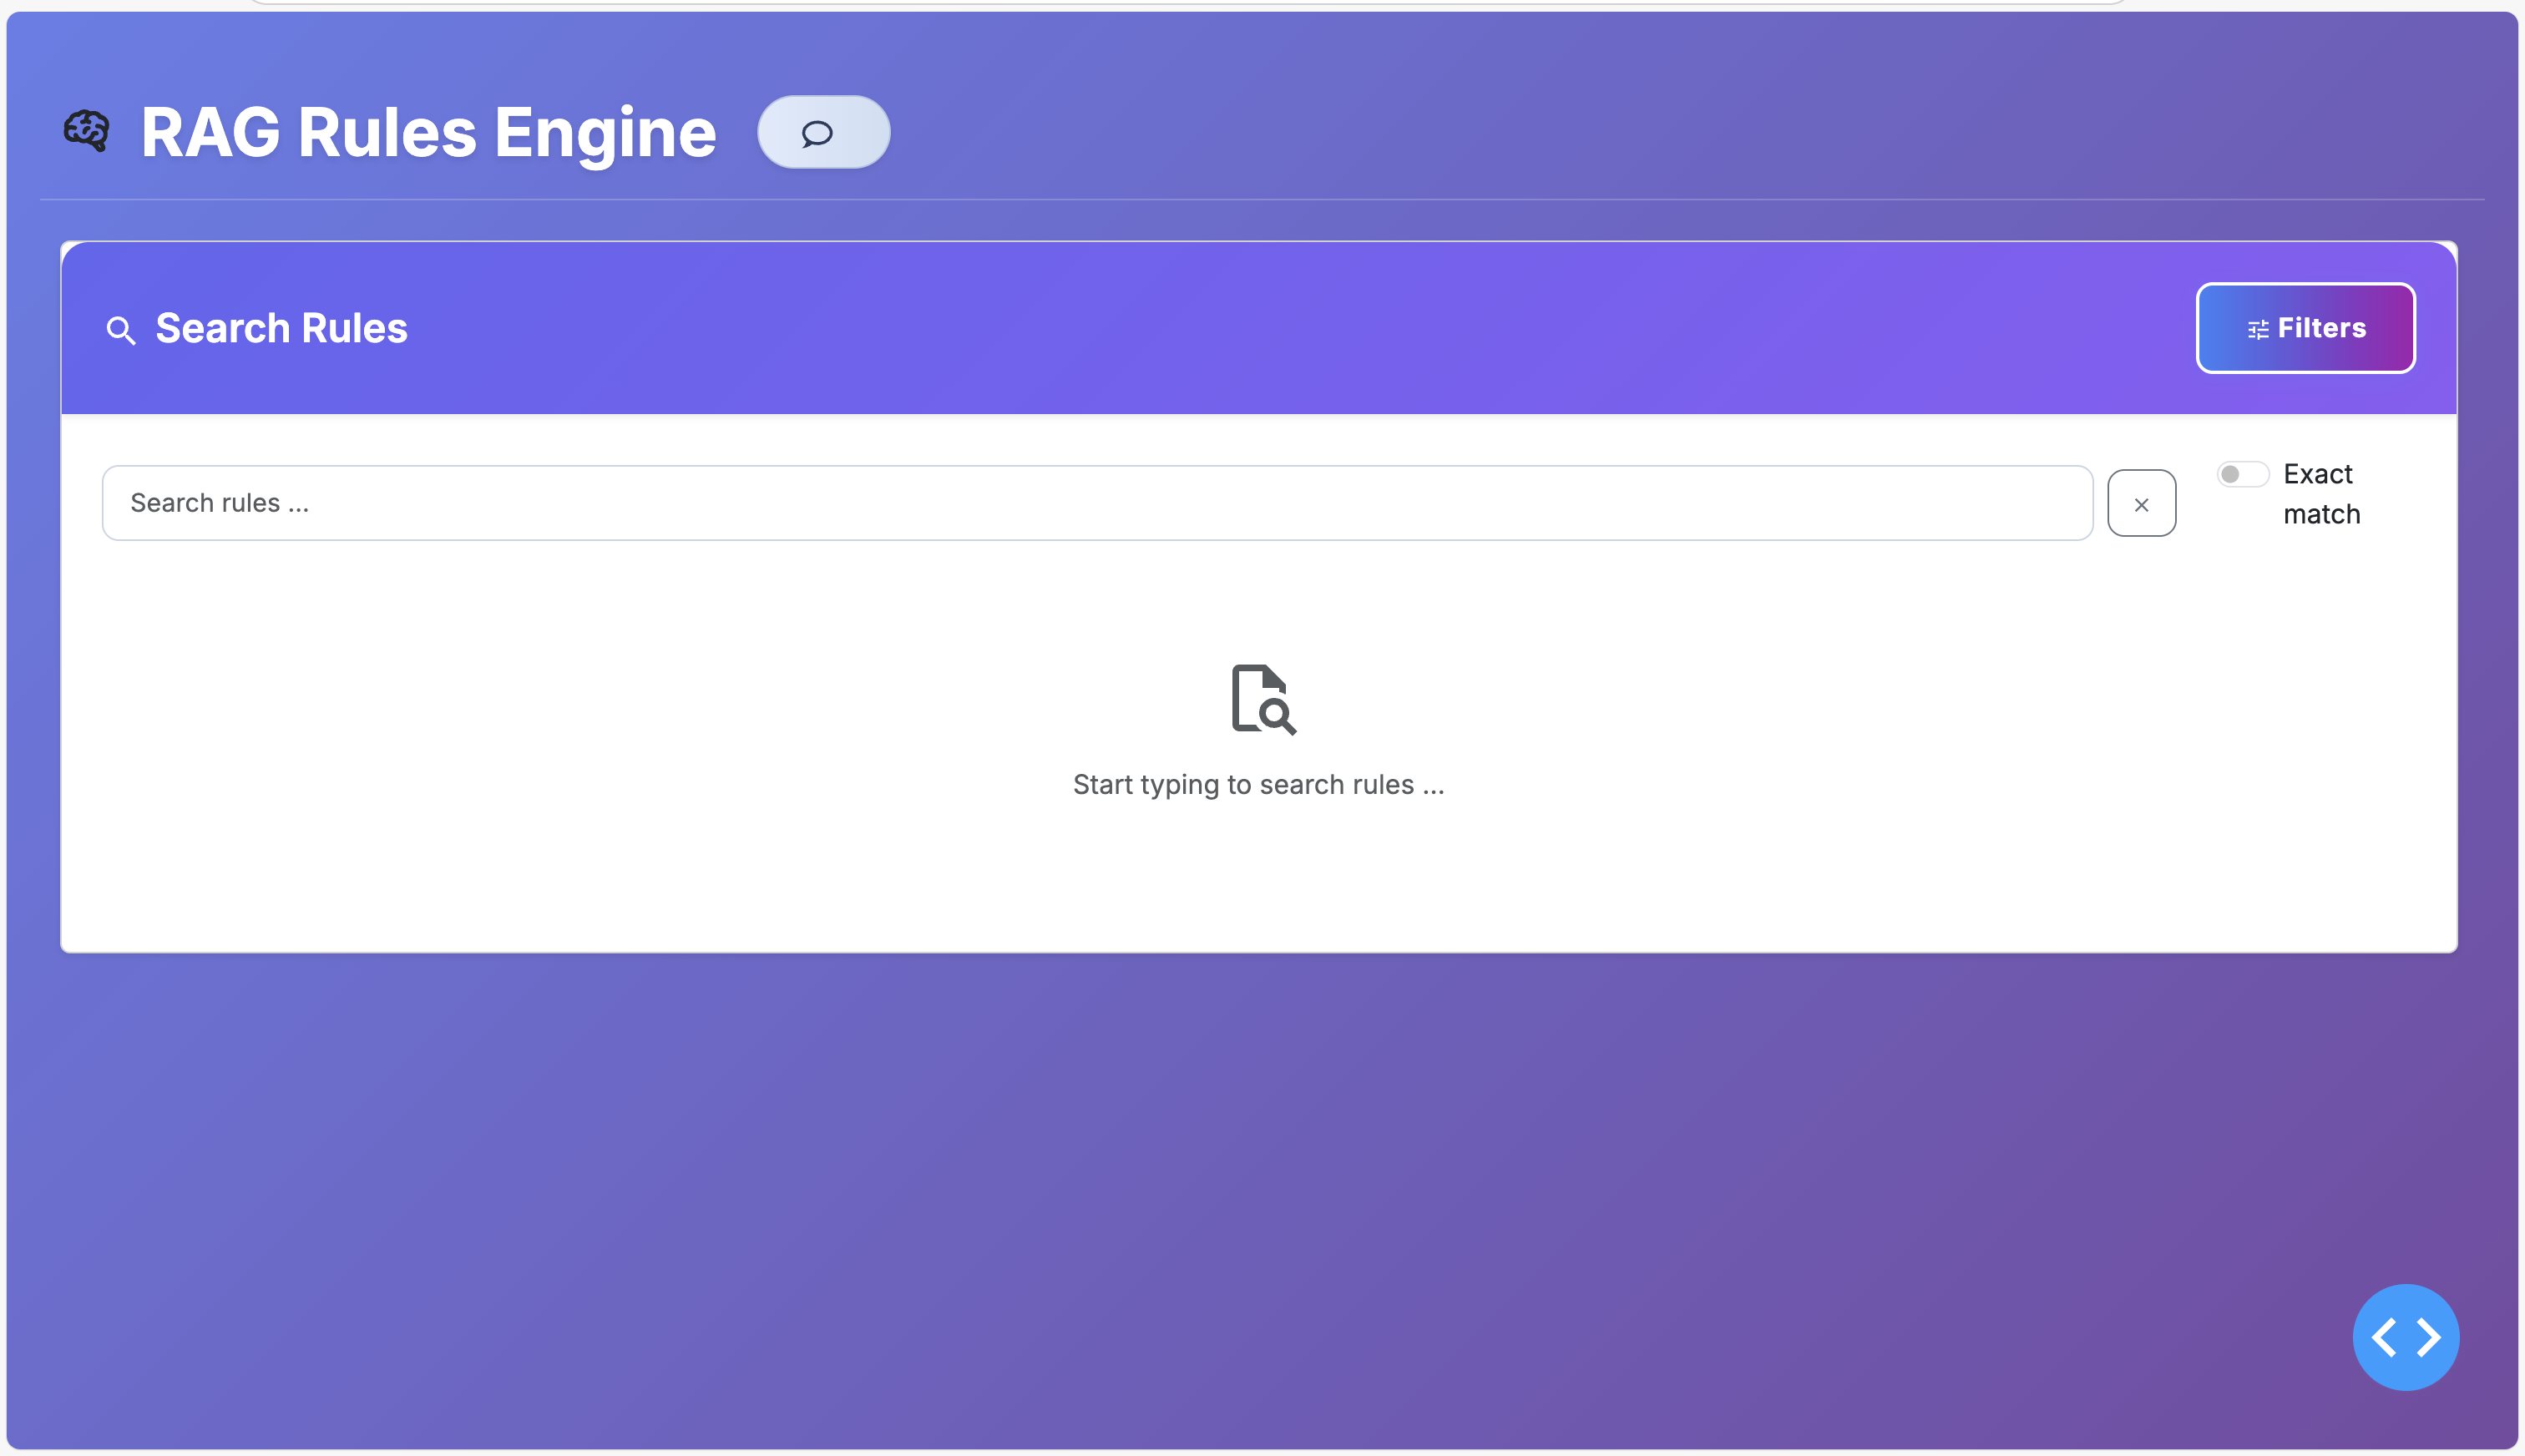
\includegraphics[width=0.9\textwidth]{Figures/full_search.png}
\captionof{figure}{Search interface with query input, mode toggle (Keyword/Hybrid), and filter panel.}\label{fig:search-interface}
\end{minipage}
\vspace{0.5em}

\subsection{Faceted Filtering}

\vspace{0.5em}
\noindent
\begin{minipage}{\textwidth}
\centering
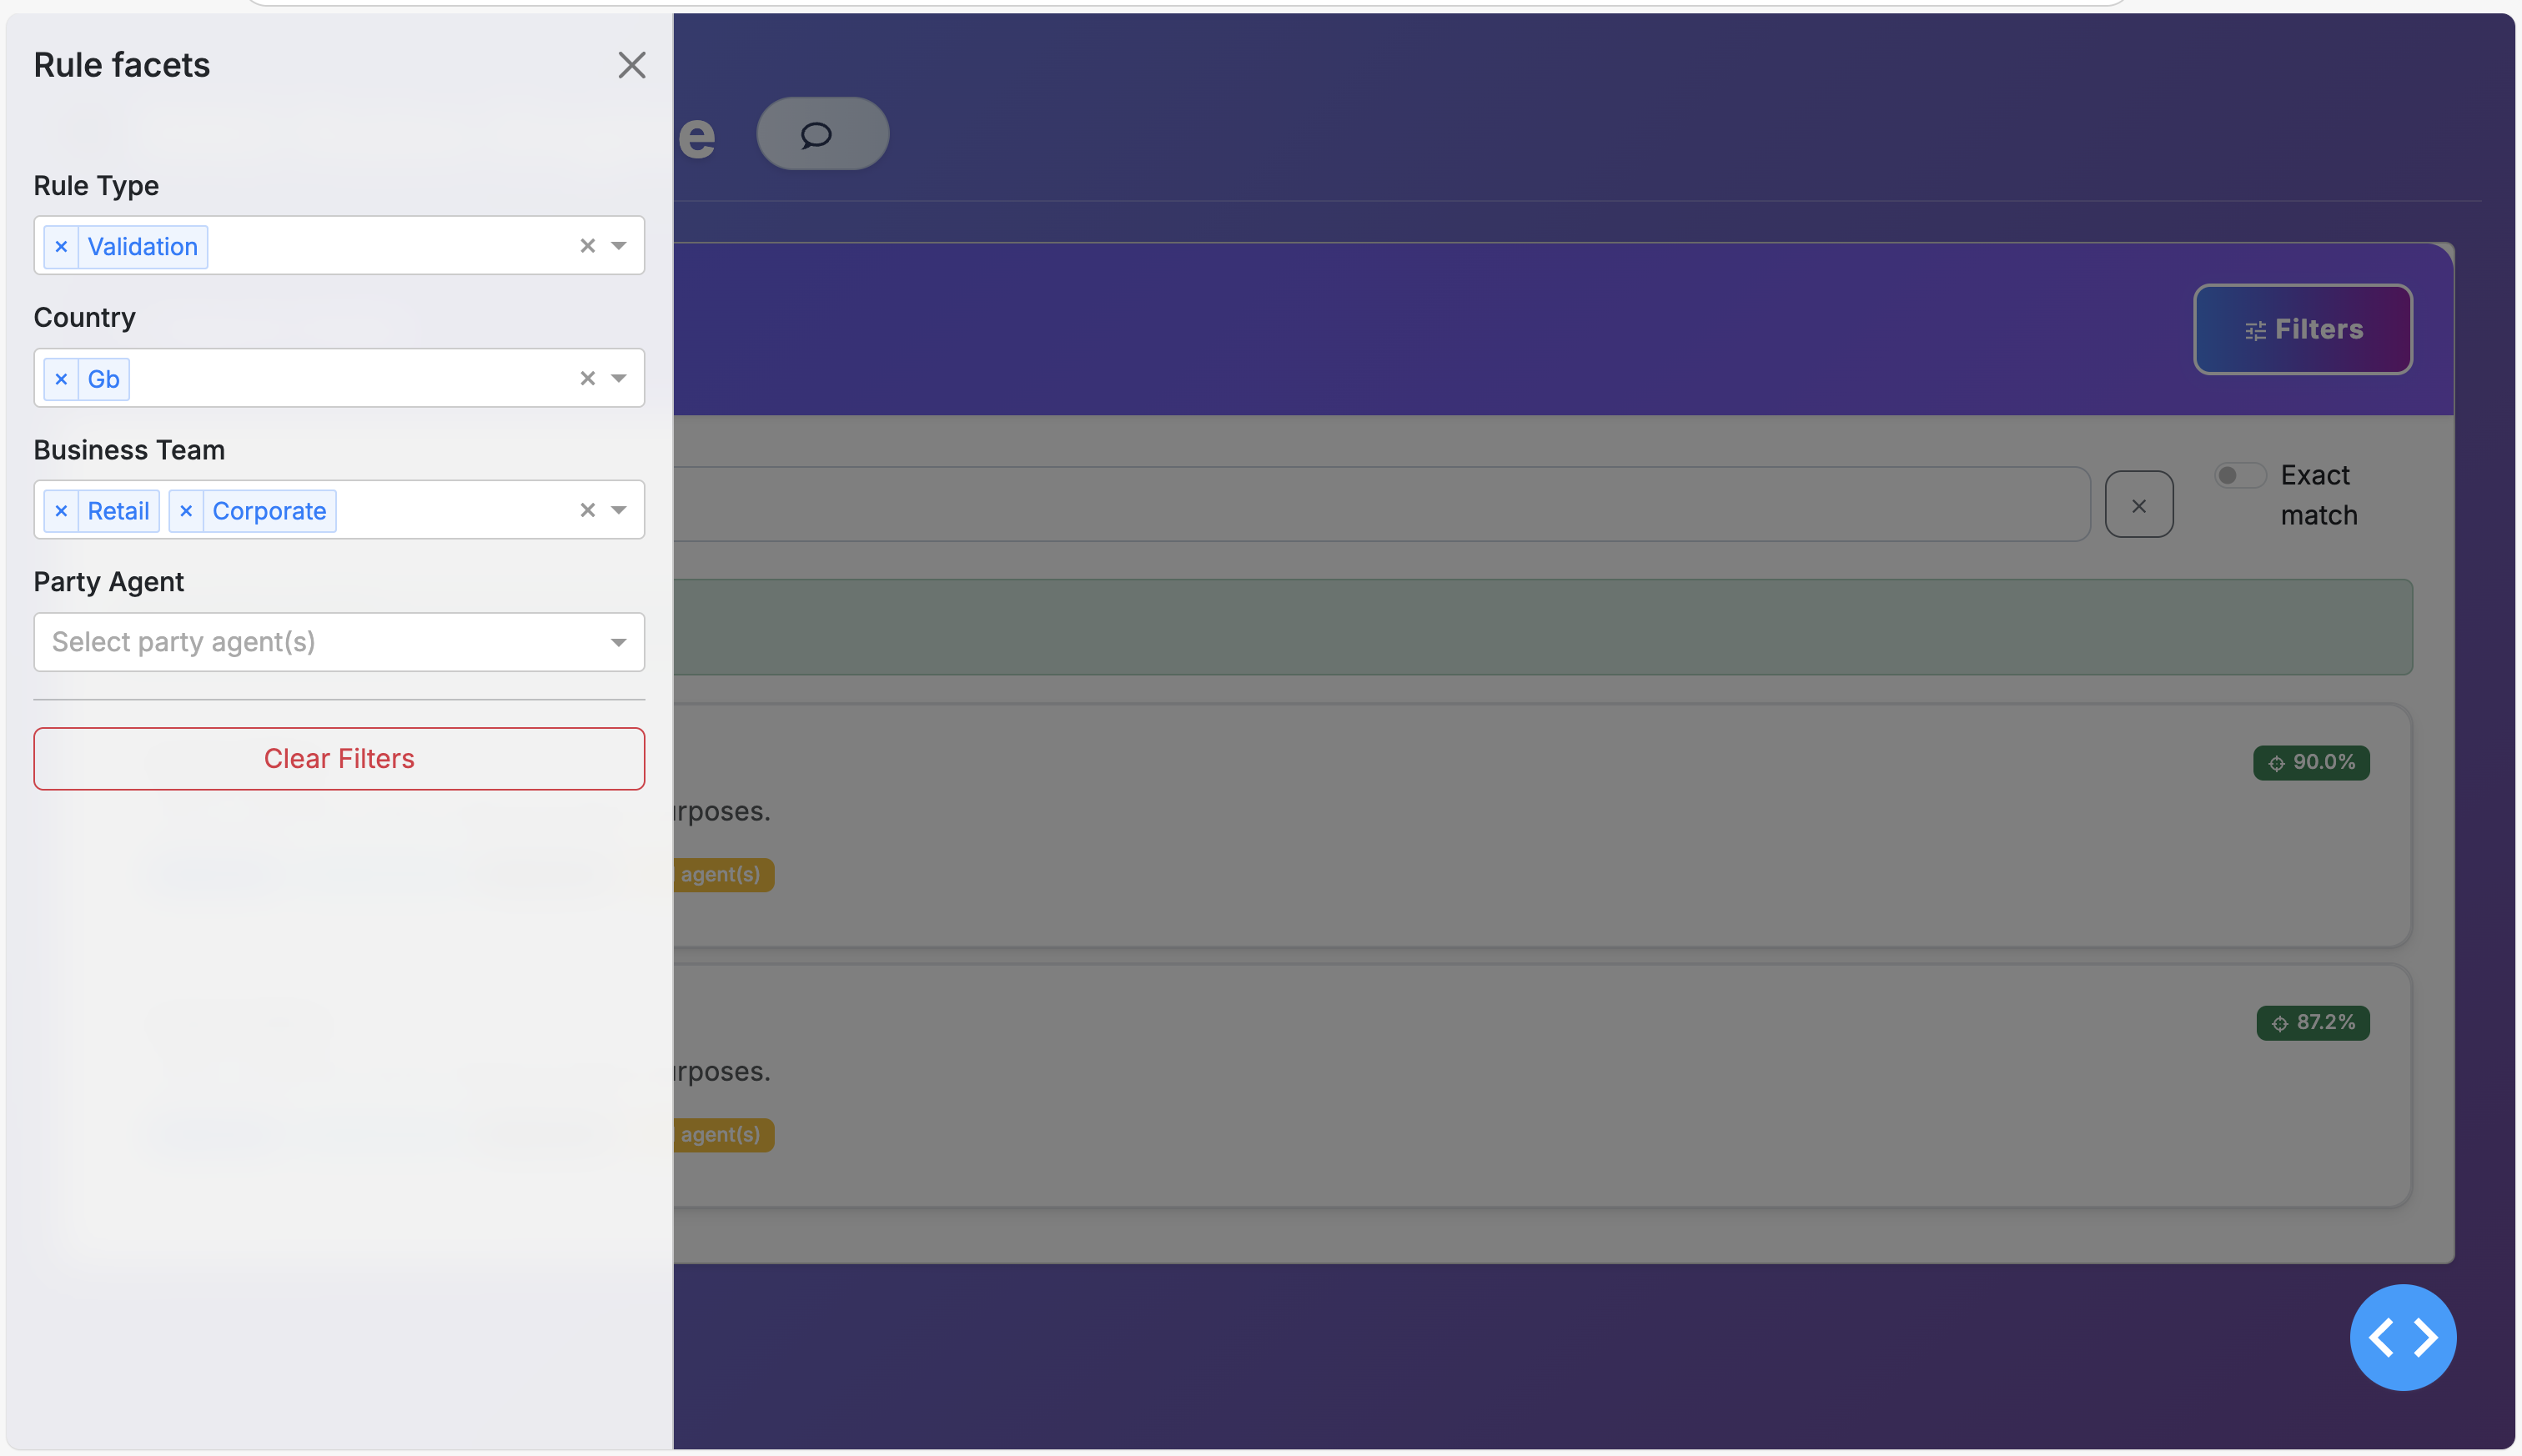
\includegraphics[width=0.9\textwidth]{Figures/search_filters.png}
\captionof{figure}{Multi-select filtering across Rule Type, Country, Business Type, and Party Agent.}\label{fig:search-filters}
\end{minipage}
\vspace{0.5em}

\subsection{Search Results}

\vspace{0.5em}
\noindent
\begin{minipage}{\textwidth}
\centering
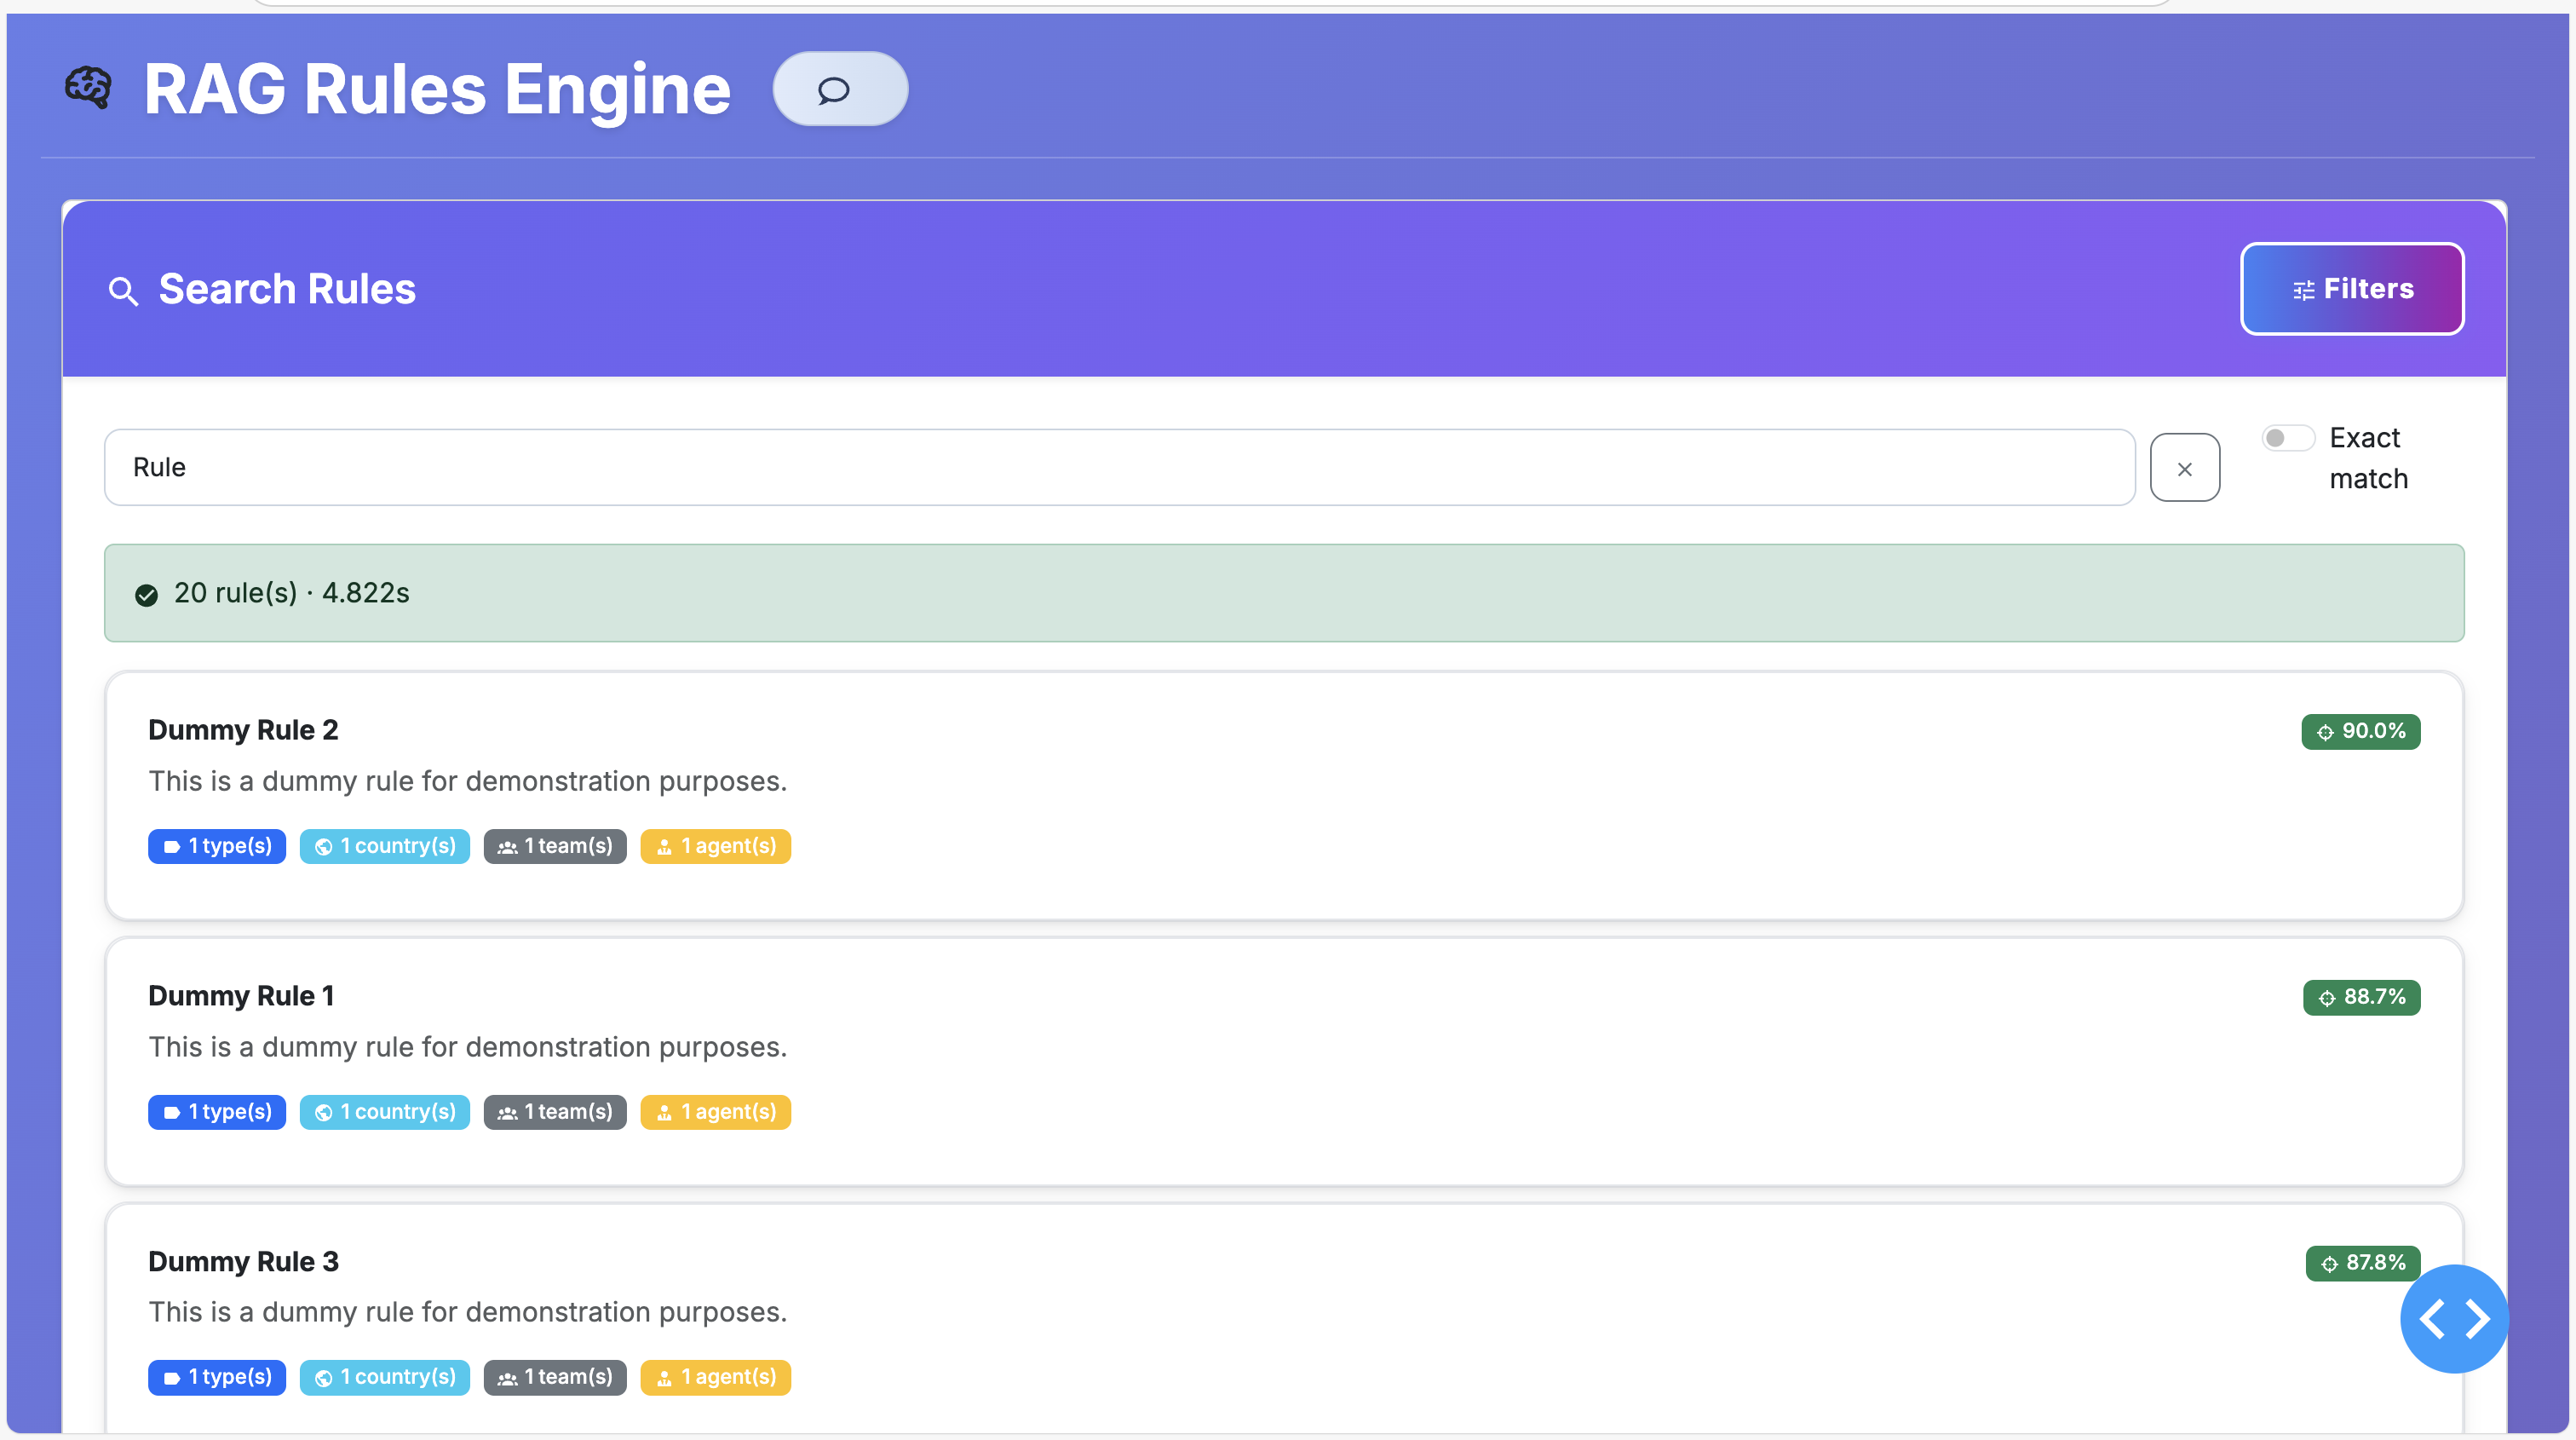
\includegraphics[width=0.9\textwidth]{Figures/full_search_results.png}
\captionof{figure}{Ranked rule cards with similarity scores and categorical badges.}\label{fig:search-results}
\end{minipage}
\vspace{0.5em}

\subsection{Rule Details}

\vspace{0.5em}
\noindent
\begin{minipage}{\textwidth}
\centering
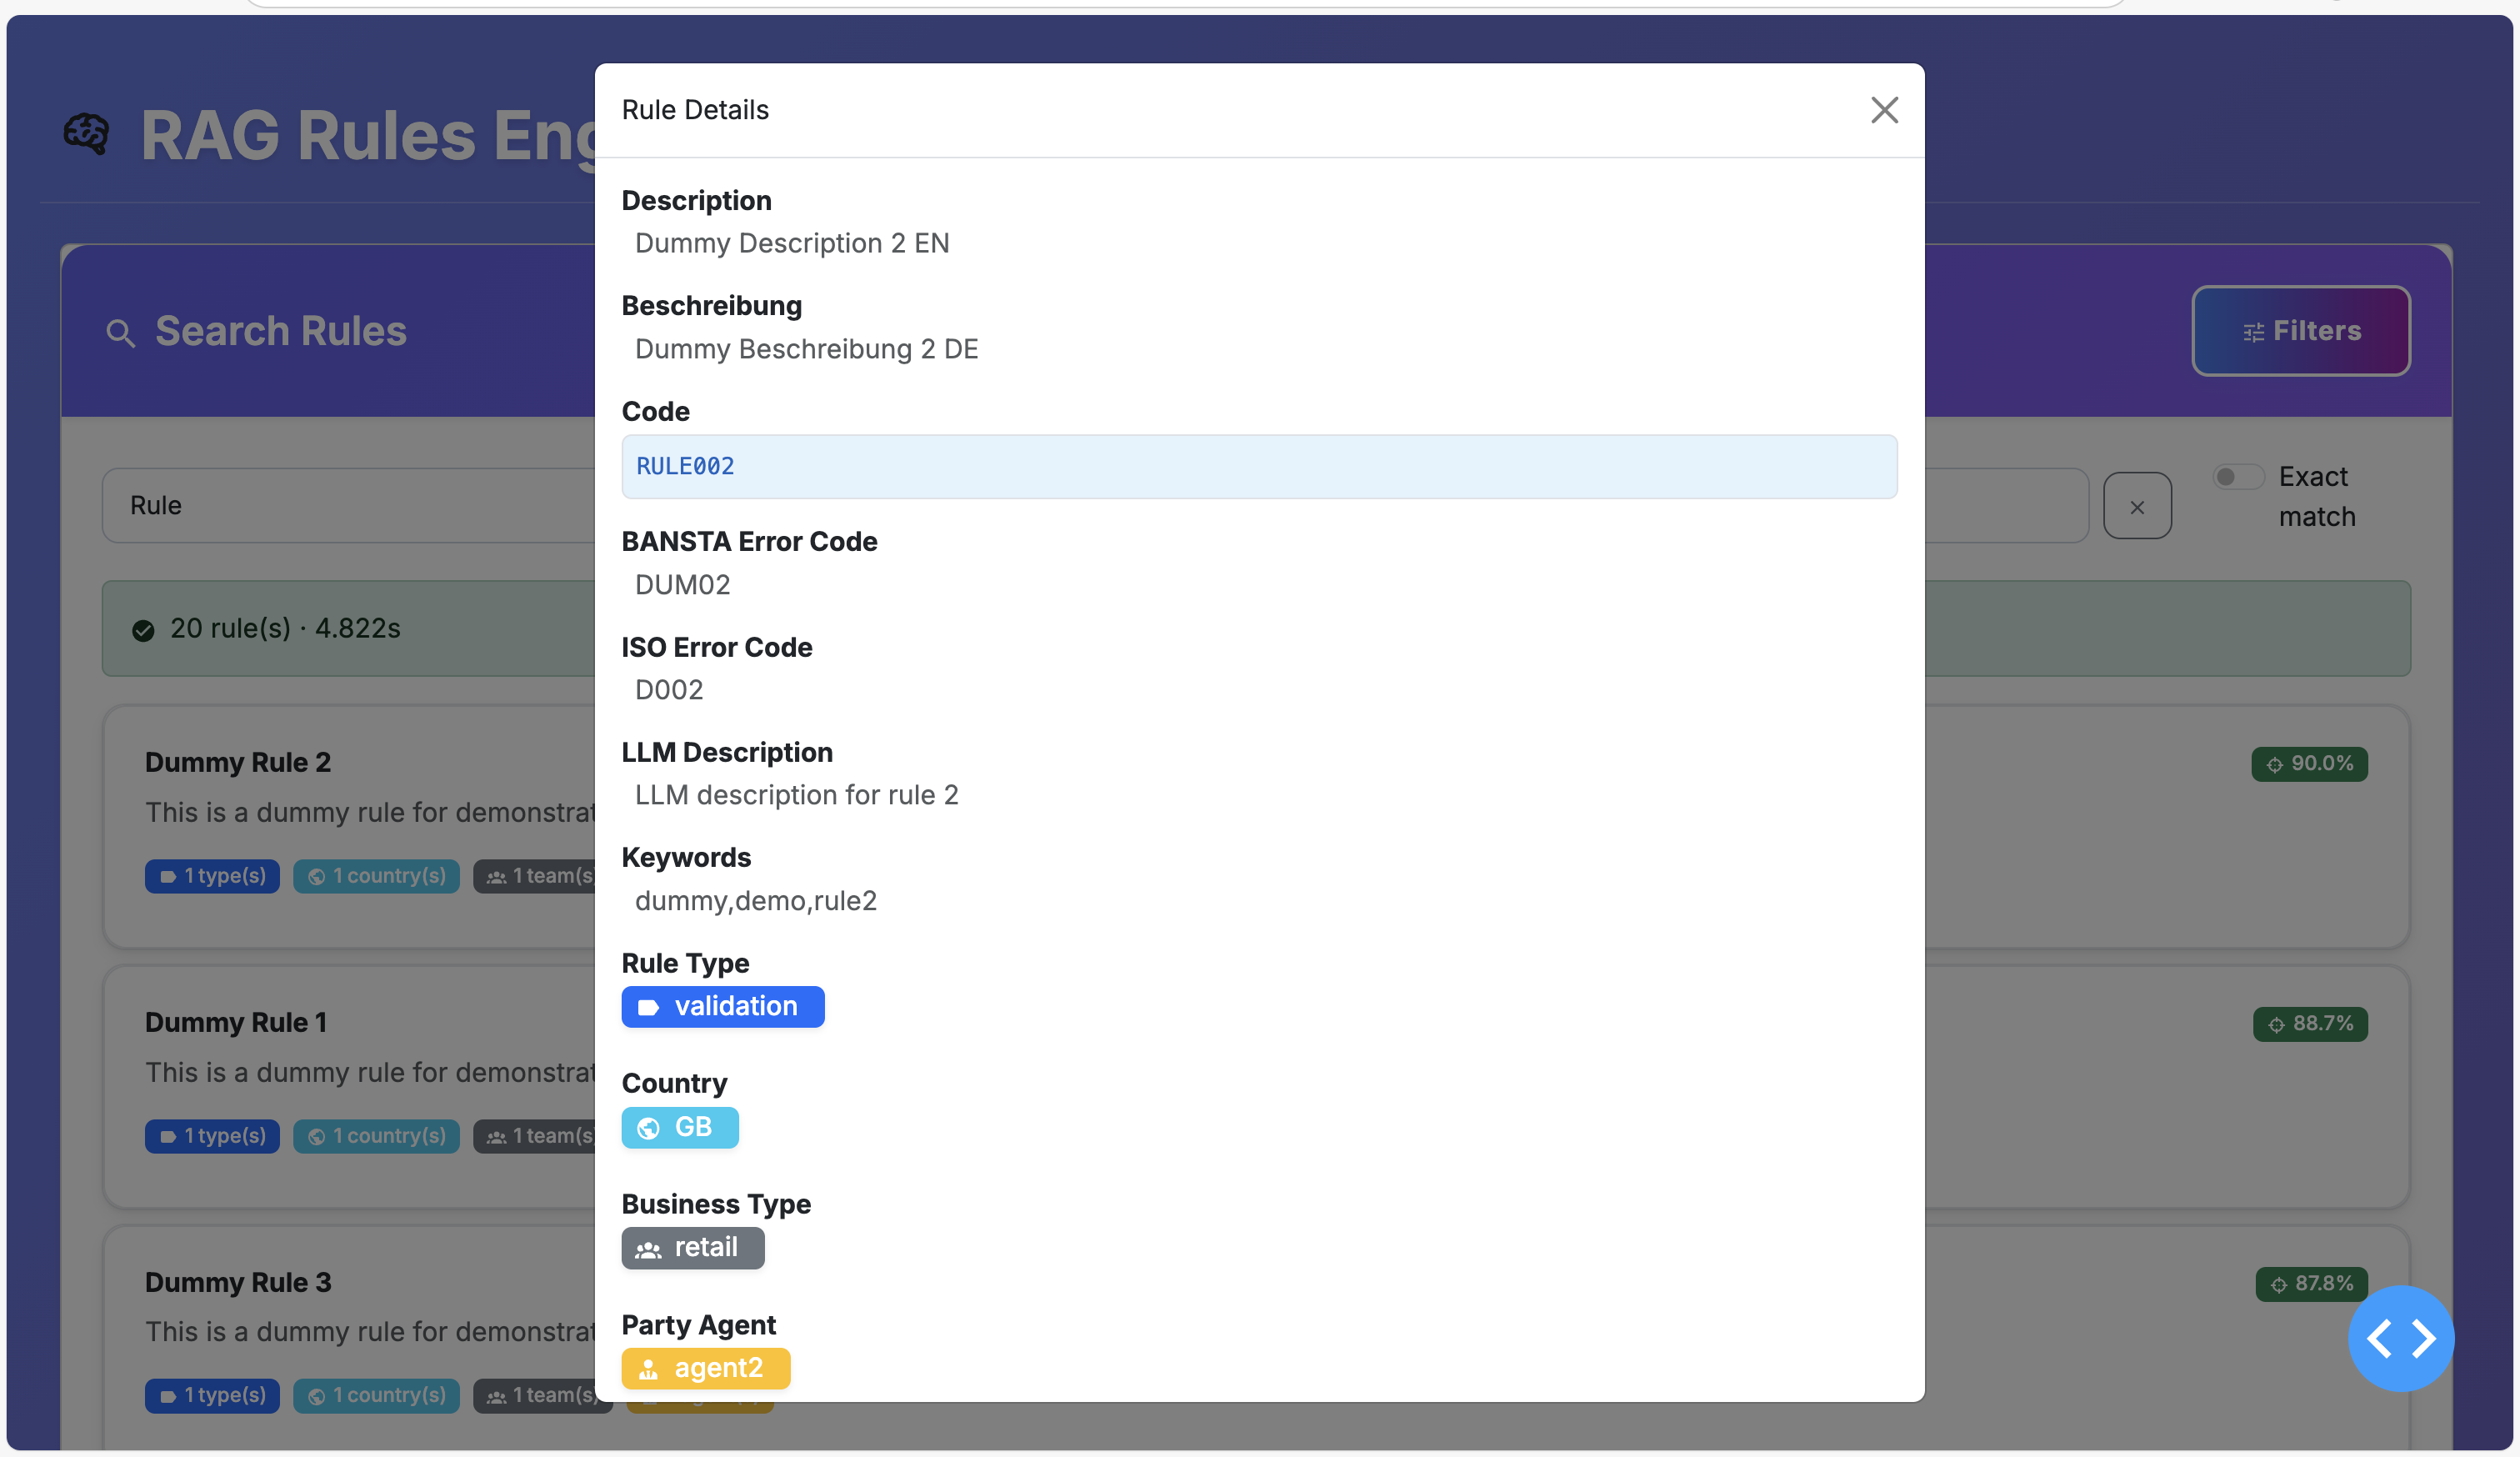
\includegraphics[width=0.85\textwidth]{Figures/rule_details.png}
\captionof{figure}{Detailed rule view with code, descriptions, and metadata.}\label{fig:rule-details}
\end{minipage}
\vspace{0.5em}

\subsection{Unified Interface}

\vspace{0.5em}
\noindent
\begin{minipage}{\textwidth}
\centering
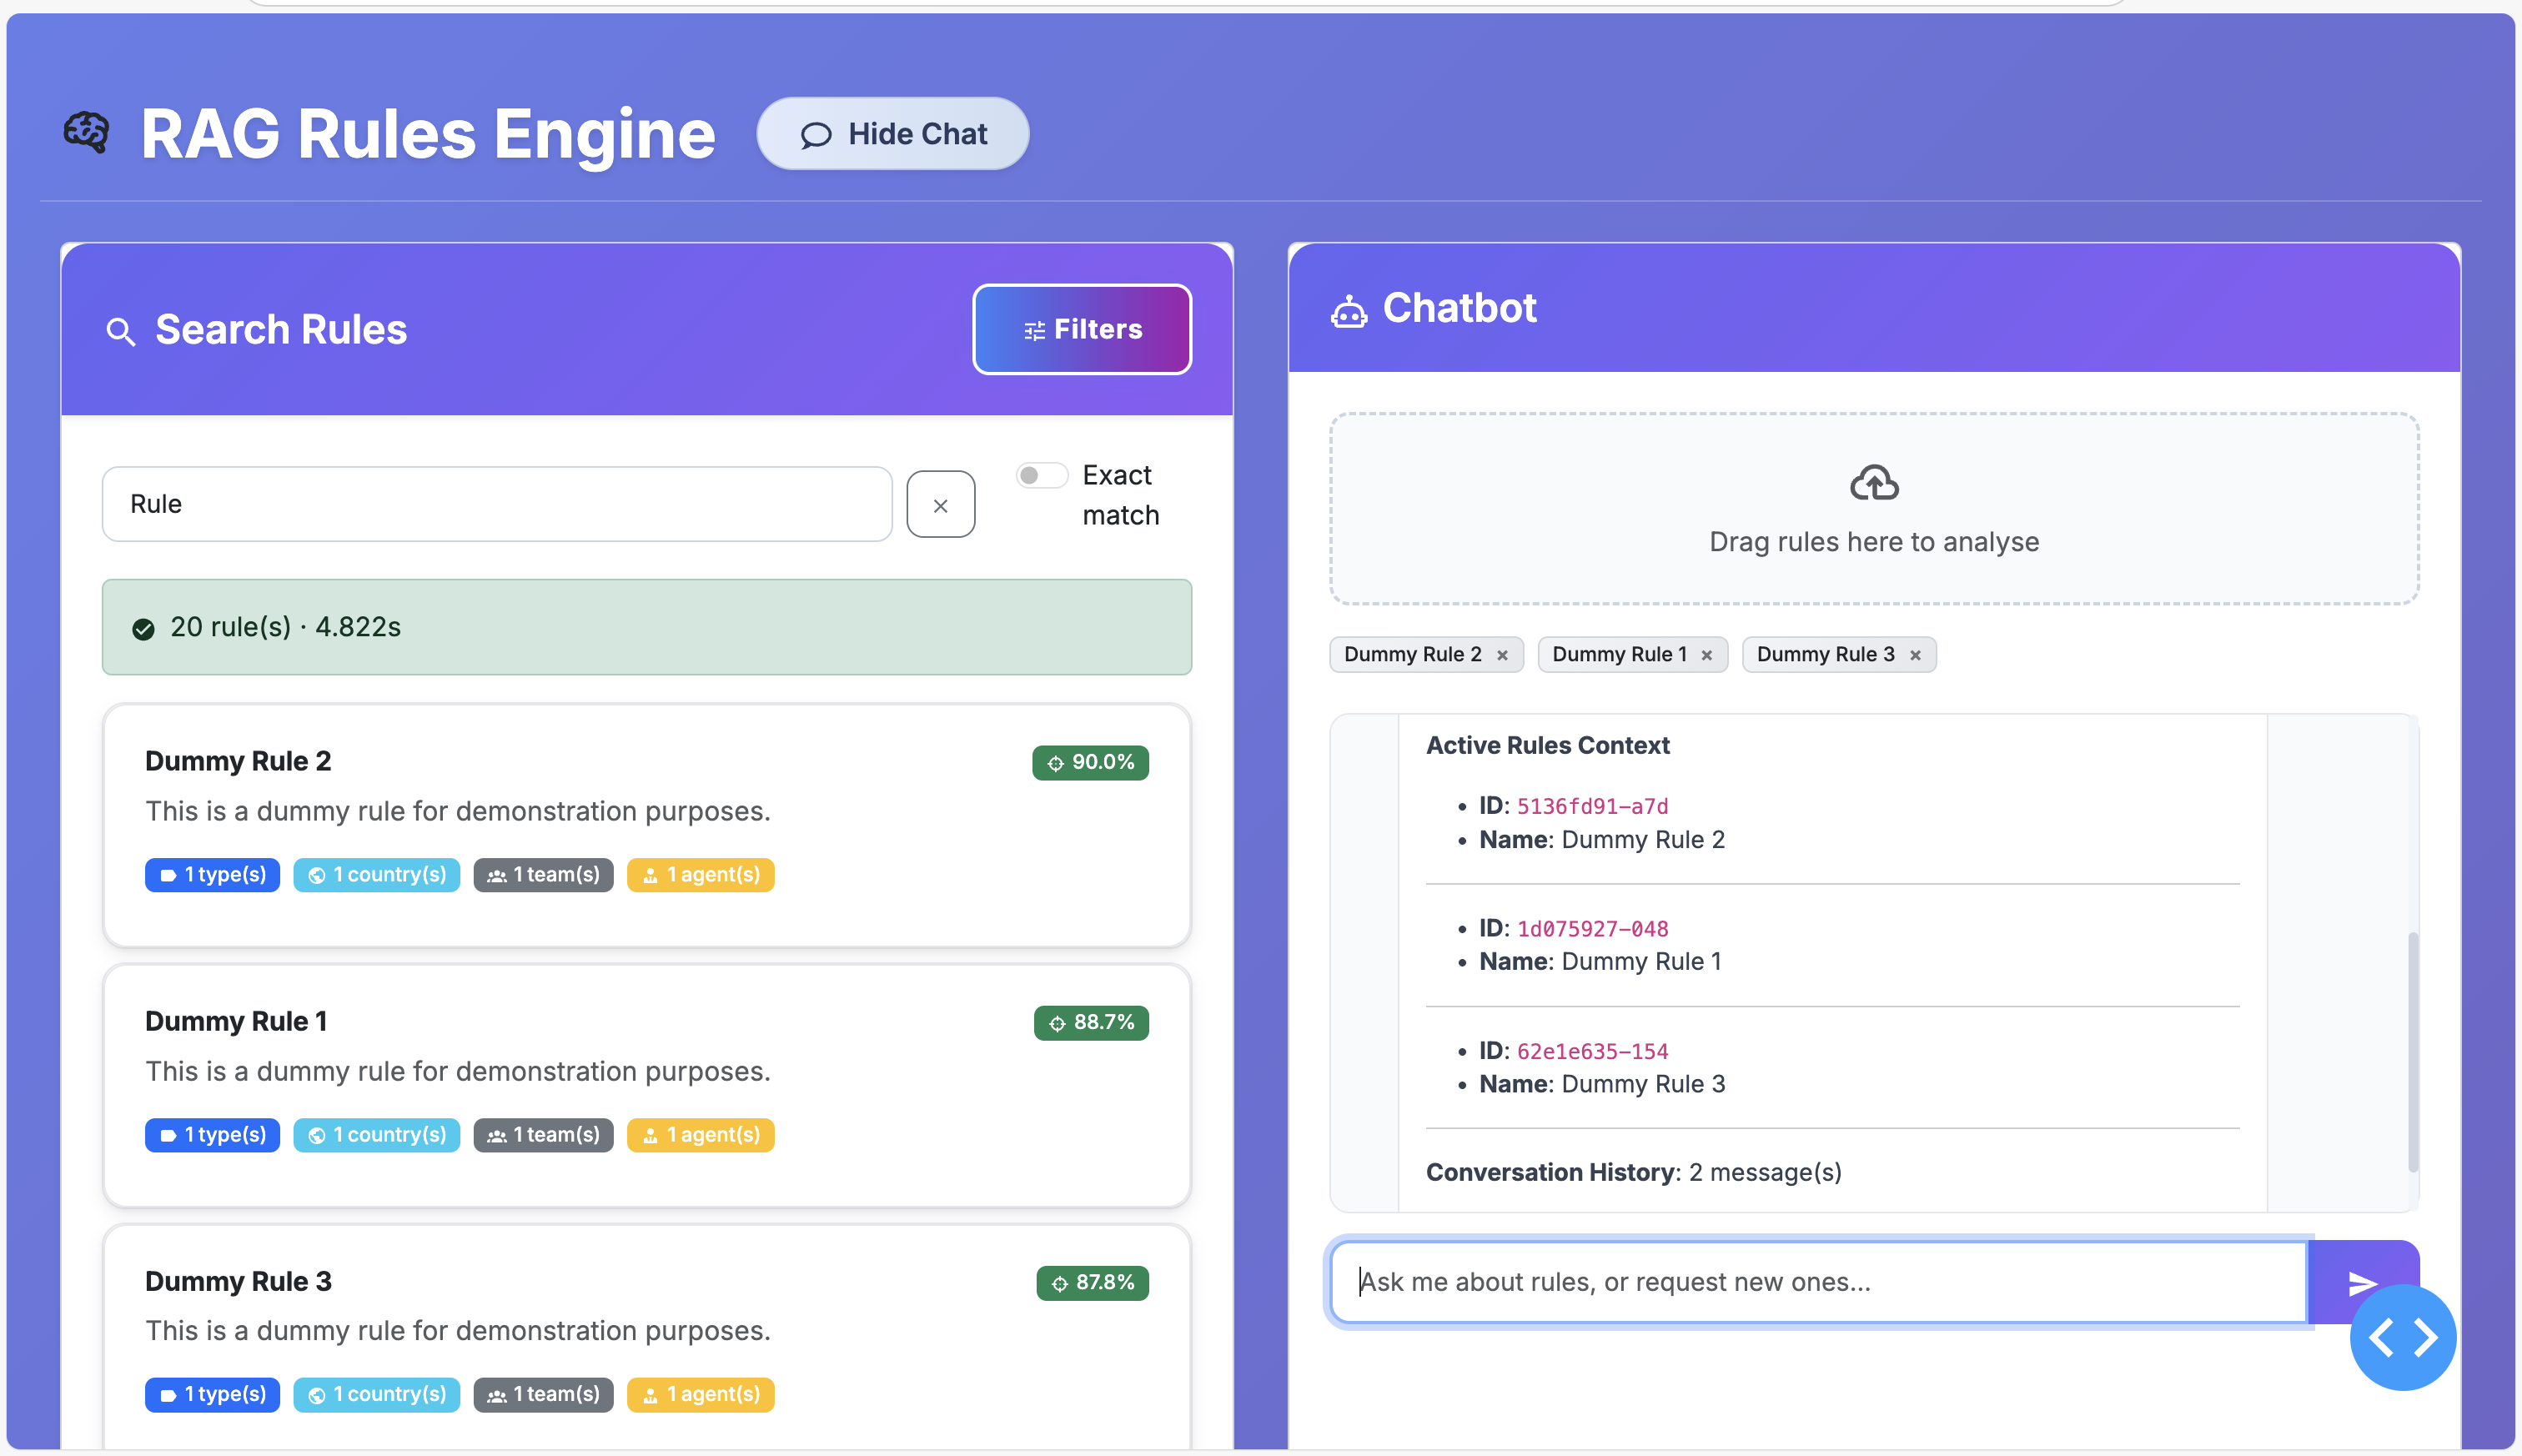
\includegraphics[width=0.95\textwidth]{Figures/search_chat_example.png}
\captionof{figure}{Combined search and conversational exploration interface.}\label{fig:search-chat}
\end{minipage}
\vspace{0.5em}

\section{Summary}

The implementation demonstrates that sophisticated RAG capabilities can be delivered through pragmatic engineering within banking constraints. Key achievements include:

\begin{itemize}[leftmargin=*,itemsep=2pt,topsep=2pt]
  \item Three complementary retrieval signals with empirically tuned weights (80\% semantic, 10\% BM25, 10\% fuzzy)
  \item Parallel index construction at startup for semantic and BM25, with fuzzy computed at query time
  \item Attention-aware embeddings ensuring accurate semantic representation
  \item Efficient score fusion through max normalization maintaining convex weight properties
  \item Complete retrieval pipeline in approximately 1,500 lines of core Python
\end{itemize}

By building only necessary indices at startup and computing fuzzy scores at query time, we balance initialization speed with query performance. The system achieves production-ready retrieval while maintaining simplicity and auditability required for banking deployment.
